\chapter{Neuronale Netzwerke}

Unter einem neuronalen Netzwerk versteht man ein System
aus Neuronen. Diese sind schichtweise organisiert wobei
jedes Neuron einer Schicht jeweils zu allen Neuronen der
direkt anliegenden Schichten verbunden ist.
Abbildung \ref{fig:Neuronales Netzwerk} zeigt beispielhaft ein
neuronales Netzwerk aus 19 Neuronen mit insgesamt 5 Schichten.
\bigskip

\begin{figure}[h]
    \begin{center}
        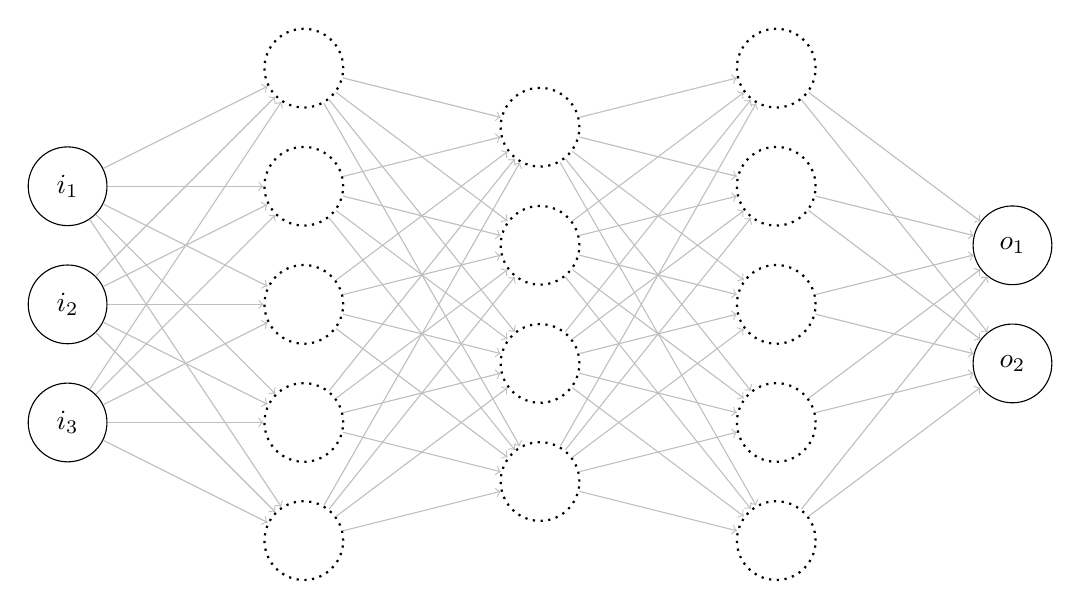
\begin{tikzpicture}[y=-1.5cm,x=3cm]
            \tikzset{
                netnode/.style={circle,draw=black,minimum size=1cm},
                hidden/.style={dotted,thick}
            }
            \node[netnode] (i1) at (0,0) {$i_1$};
            \node[netnode] (i2) at (0,1) {$i_2$};
            \node[netnode] (i3) at (0,2) {$i_3$};

            \node[netnode,hidden] (l11) at (1,-1) {};
            \node[netnode,hidden] (l12) at (1,0) {};
            \node[netnode,hidden] (l13) at (1,1) {};
            \node[netnode,hidden] (l14) at (1,2) {};
            \node[netnode,hidden] (l15) at (1,3) {};

            \node[netnode,hidden] (l21) at (2,-0.5) {};
            \node[netnode,hidden] (l22) at (2,0.5) {};
            \node[netnode,hidden] (l23) at (2,1.5) {};
            \node[netnode,hidden] (l24) at (2,2.5) {};

            \node[netnode,hidden] (l31) at (3,-1) {};
            \node[netnode,hidden] (l32) at (3,0) {};
            \node[netnode,hidden] (l33) at (3,1) {};
            \node[netnode,hidden] (l34) at (3,2) {};
            \node[netnode,hidden] (l35) at (3,3) {};

            \node[netnode] (o1) at (4,0.5) {$o_1$};
            \node[netnode] (o2) at (4,1.5) {$o_2$};

            \foreach \i in {1,2,3}{
                    \foreach \j in {1,...,5}{
                            \draw[->,black!25] (i\i) -- (l1\j);
                        }
                }
            \foreach \i in {1,...,5}{
                    \foreach \j in {1,...,4}{
                            \draw[->,black!25] (l1\i) -- (l2\j);
                        }
                }
            \foreach \i in {1,...,4}{
                    \foreach \j in {1,...,5}{
                            \draw[->,black!25] (l2\i) -- (l3\j);
                        }
                }
            \foreach \i in {1,...,5}{
                    \foreach \j in {1,2}{
                            \draw[->,black!25] (l3\i) -- (o\j);
                        }
                }
        \end{tikzpicture}
    \end{center}
    \caption{Struktur eines neuronalen Netzwerks}
    \label{fig:Neuronales Netzwerk}
\end{figure}

\section{Neuronen}\label{sec:neuronen}

Unter einem Neuron versteht sich bei neuronalen Netzen lediglich ein Knoten,
in dem üblicherweise ein 32-bit großer Wert hinterlegt ist. Häufig kommen hier
Gleitkommazahlen zwischen -1.0 und 1.0 zum Einsatz, da sich dieser Wertebereich
besonders gut zum Rechnen eignet und Eigenschaften bezüglich der
Multiplikation besitzt, die eine Wertexplosion verhindern.
Die Werte aller Neuronen, mit Ausnahme derer in der Eingabeschicht, setzen sich
jeweils aus den Werten aller Neuronen der direkt davor liegenden Schicht zusammen.
Das genaue Vorgehen bei der Wertermittlung hängt jeweils vom Netzwerk
und den dort verwendeten Aktivierungsfunktionen ab.

\section{Schichten und Kanten}\label{sec:schichtenundkanten}

In einem neuronalen Netzwerk ist jedes Neuron einer Schicht mit allen Neuronen
der jeweiligen davor liegenden und danach liegenden Schicht über Kanten verbunden.
Neuronale Netzwerke sind unidirektionale Graphen, demnach fließen Informationen
über Schichten (und folglich Kanten) nur in eine Richtung.

Allen Kanten wird initial eine Gewichtung zugewiesen, welche erneut
netzwerkabgängig generiert werden oder durch zuvor angelernte Daten bestimmt
werden. Beim Trainieren des Netzwerks werden diese bei jeder Lerniteration
(auch \emph{Epoch} genannt) justiert, während sie beim Betrieb für gewöhnlich
keine Änderungen mehr erfahren.
Die Genauigkeit eines Netzwerks wird überwiegend durch diese Gewichte bestimmt,
daher ist das Ziel beim Trainieren eines Netzes die Optimierung jener.

Kantengewichte wirken sich maßgeblich auf die Wertberechnung von Neuronen aus.
Diese wird in zwei Schritten ausgeführt. Im ersten Schritt wird aus den
Kantengewichten aller eingehenden Kanten und den Werten der darüber
verbundenen Neuronen die Produktsumme gebildet.
Für den zweiten Schritt sind jeweils Aktivierungsfunktionen notwendig, welche
im nachfolgenden Kapitel erläutert werden.

\section{Aktivierungsfunktionen}\label{sec:aktivierungsfunktionen}

Im zweiten Schritt wird der zuvor errechnete Wert durch eine weitere Funktion
modifiziert. Sogenannte \emph{Aktivierungsfunktionen} können beliebig gewählt
werden, müssen jedoch offensichtlich alle möglichen Eingaben auf einen Wert
abbilden können. Die verwendete Aktivierungsfunktion kann je nach
Schicht variieren. Einmal gewählt, ist diese jedoch für die jeweilige Schicht
im Netzwerk für die Laufzeit fest.

Die beiden erläuterten Berechnungsschritte werden schichtweise in Richtung des
Datenflusses des Netzwerks für alle Neuronen durchgeführt. Im folgenden
Beispiel wird bildhaft dargestellt, wie solch eine Neuronenwertberechnung für
ein Netzwerk aussieht, welche in der betrachteten Schicht die
$tanH$-Aktivierungsfunktion verwendet.

\begin{figure}
    \centering
    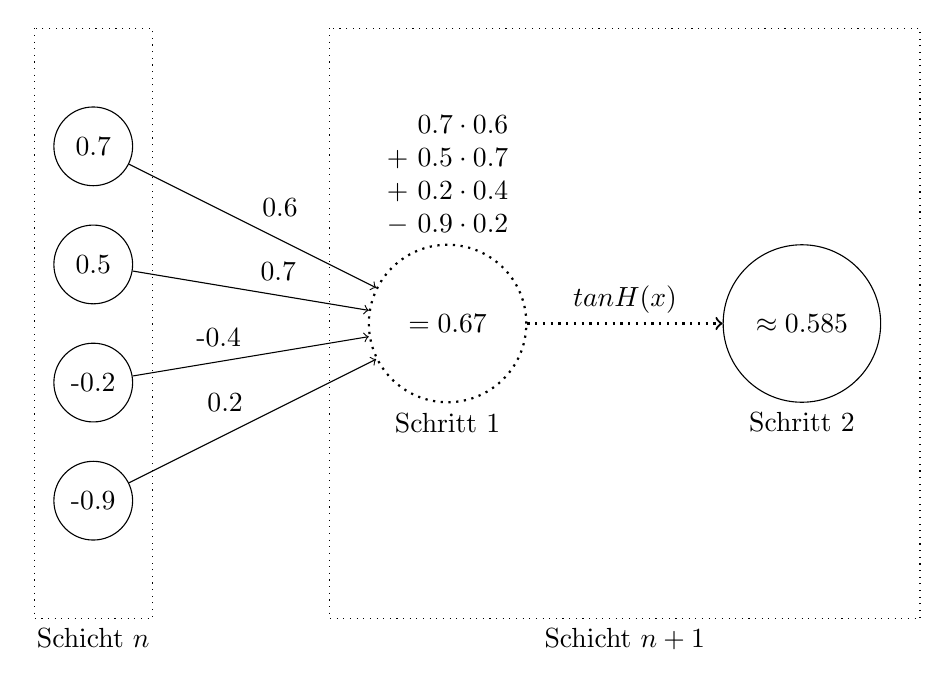
\begin{tikzpicture}[y=-1.5cm,x=1.5cm]
        \tikzset{
            netnode/.style={circle,draw=black,minimum size=1cm},
            hidden/.style={dotted,thick}
        }
        \node[netnode] (i1) at (0,0) {0.7};
        \node[netnode] (i2) at (0,1) {0.5};
        \node[netnode] (i3) at (0,2) {-0.2};
        \node[netnode] (i4) at (0,3) {-0.9};

        \draw[draw=black,dotted] (-0.5,-1) rectangle ++(1,5) ++(-0.5,0) node[below] {Schicht $n$};
        \draw[draw=black,dotted] (2,-1) rectangle ++(5,5) ++(-2.5,0) node[below] {Schicht $n+1$};

        \node[netnode,minimum size=2cm,dotted,thick] (o1) at (3,1.5) [label=below:Schritt 1] {$=0.67$};
        \node (o1l) [above of=o1,align=right,above] {$0.7\cdot 0.6$\\$+\ 0.5\cdot 0.7$\\$+\ 0.2\cdot 0.4$\\$-\ 0.9\cdot 0.2$};

        \node[netnode,minimum size=2cm] (o2) at (6,1.5) [label=below:Schritt 2] {$\approx 0.585$};

        \draw[->] (i1) -- node[auto] {0.6} (o1);
        \draw[->] (i2) -- node[auto] {0.7} (o1);
        \draw[->] (i3) -- node[auto] {-0.4} (o1);
        \draw[->] (i4) -- node[auto] {0.2} (o1);
        \draw[->,dotted,thick] (o1) -- node[above] {$tanH(x)$} (o2);
    \end{tikzpicture}
    \caption{Berechnung eines Neuronenwertes\\mit der $tanH$ Aktivierungsfunktion}
\end{figure}

Die Wahl der Aktivierungsfunktion beeinflusst die möglichen
Werte, die Neuronen innerhalb einer Schicht annehmen können. Um eine
Wertexplosion zu vermeiden (z.B. bei Verwendung von $ReLU(x): \max(0,x)$ als
Aktivierungsfunktion), können zusätzliche Normalisierungsschichten verwendet
werden, welche die Neuronenwerte einer Schicht auf einen erwünschten Zielbereich
einschränken. Es existieren jedoch auch Aktivierungsfunktionen, die diese
\emph{Squashing-}Eigenschaft direkt besitzen. Darunter zählt auch die im
vorherigen Beispiel verwendetete Funktion $tanH$, bei der alle Eingaben auf den
Zielbereich [-1,1] abgebildet werden.

Im Folgenden sind sind einige, für neuronale Netzwerke übliche
Aktivierungsfunktionen abgebildet.

\begin{figure}[H]
    \begin{minipage}{0.45\textwidth}
        \begin{center}
            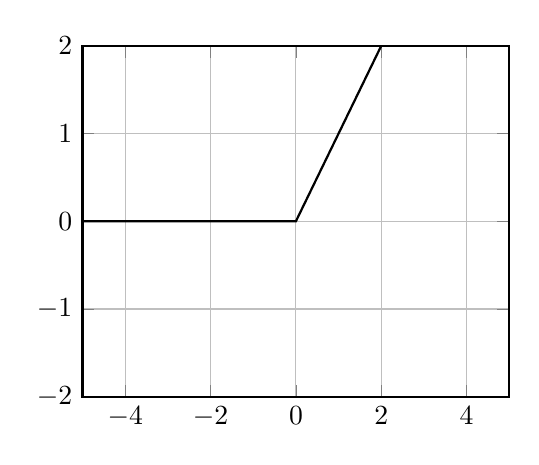
\begin{tikzpicture}
                \begin{axis}[width=7cm,xmin=-5,xmax=5,ymin=-2,ymax=2,thick,grid=both]
                    \addplot[] {max(x,0))};
                \end{axis}
            \end{tikzpicture}
        \end{center}
        \caption{ReLU}
    \end{minipage}\hfill
    \begin{minipage}{0.45\textwidth}
        \begin{center}
            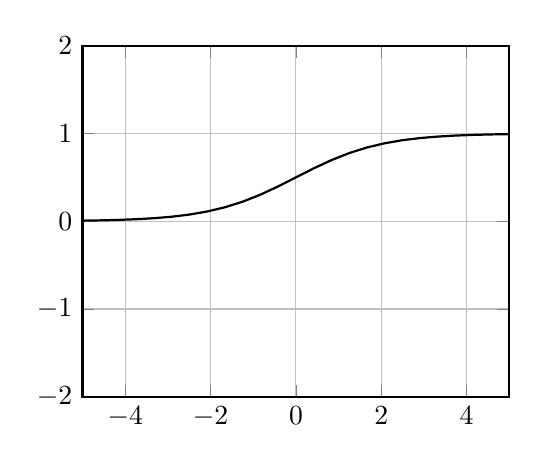
\begin{tikzpicture}
                \begin{axis}[width=7cm,xmin=-5,xmax=5,ymin=-2,ymax=2,thick,grid=both]
                    \addplot[] {1/(1+exp(-x))};
                \end{axis}
            \end{tikzpicture}
        \end{center}
        \caption{Sigmoid}
    \end{minipage}
\end{figure}
%
\begin{figure}[H]
    \begin{minipage}{0.45\textwidth}
        \begin{center}
            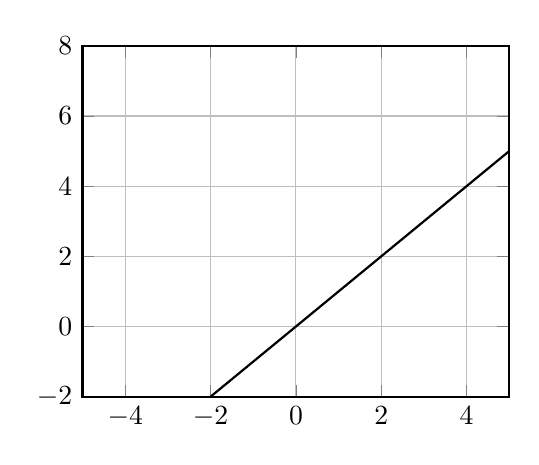
\begin{tikzpicture}
                \begin{axis}[width=7cm,xmin=-5,xmax=5,ymin=-2,ymax=8,thick,grid=both]
                    \addplot[] {x};
                \end{axis}
            \end{tikzpicture}
        \end{center}
        \caption{Softmax}
    \end{minipage}\hfill
    \begin{minipage}{0.45\textwidth}
        \begin{center}
            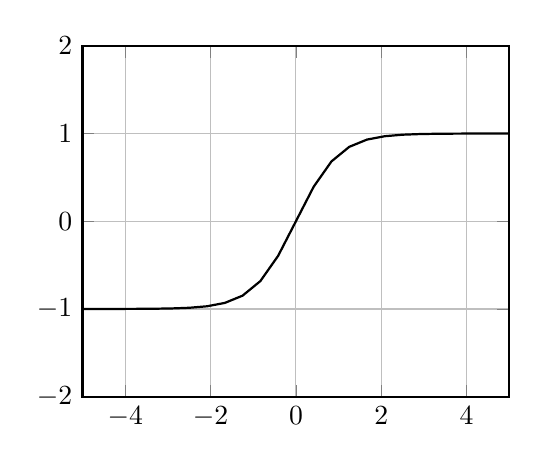
\begin{tikzpicture}
                \begin{axis}[width=7cm,xmin=-5,xmax=5,ymin=-2,ymax=2,thick,grid=both]
                    \addplot[] {(exp(x)-exp(-x)) / (exp(x)+exp(-x))};
                \end{axis}
            \end{tikzpicture}
        \end{center}
        \caption{tanH}
    \end{minipage}
\end{figure}

\section{Training}\label{sec:training}

Die Stärken und Schwächen eines neuronalen Netzwerks liegen neben der
Struktur der Neuronen, der Schichten und den gewählten Aktivierungsfunktionen
vor allem in den verwendeten Kantengewichten. Diese zu optimieren kann ein
langwieriger und rechenintensiver Prozess sein. Kleine Änderungen im Aufbau
des Netzwerks können große Teile von zuvor erlernten Gewichten unbrauchbar
machen, daher werden Netzwerke häufig an sich selbst trainiert.
Das bedeutet, dass beim Trainieren eines neuen Netzwerks die initialen
Kantengewichte keine emprischen Daten aus anderen (ähnlichen) Netzwerk verwenden,
sondern diese zu Beginn pseudozufällig gewählt werden.

\subsection{Ablauf}

Beim Training werden wiederholt verschiedene Eingaben in das Netzwerk getätigt,
zu denen das korrekte Ergebnis bekannt ist. In der letzten Schicht des Netzwerks,
der Ausgabeschicht, werden die vom Netzwerk bestimmten Werte der jeweiligen
Neuronen mit den erwarteten Werten verglichen.
Die Differenz dieser wird als Fehler bezeichnet.
Das Ziel des Trainings ist es, den Fehler durch Anpassung der Kantengewichte zu
verringern oder im Optimalfall ganz zu eliminieren (Fehler = 0).
In folgender Abbildung ist ein Fehlerbeispiel dargestellt.

\begin{figure}[H]
    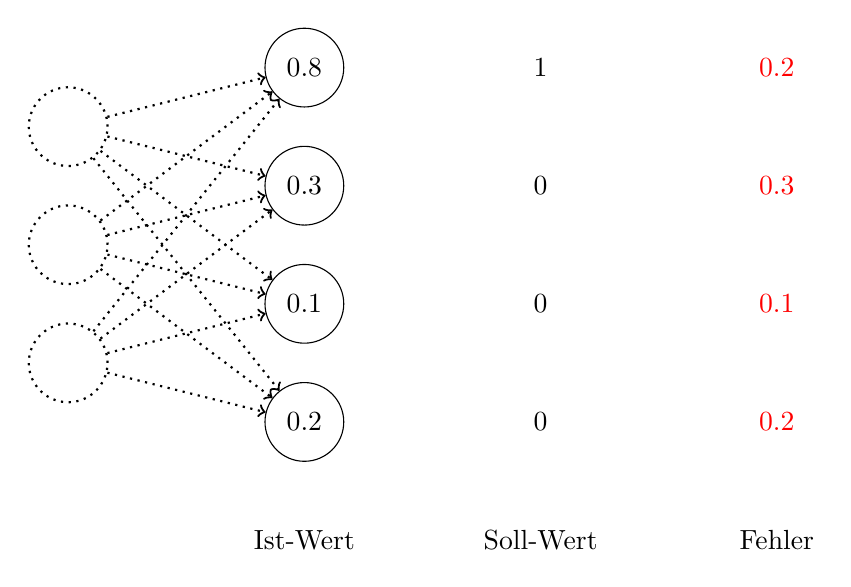
\begin{tikzpicture}[x=3cm,y=-1.5cm]
        \tikzset{
            netnode/.style={circle,draw=black,minimum size=1cm},
            hidden/.style={dotted,thick}
        }
        \node[netnode,hidden] (h1) at(0,0.5) {};
        \node[netnode,hidden] (h2) at(0,1.5) {};
        \node[netnode,hidden] (h3) at(0,2.5) {};

        \node[netnode] (o1) at (1,0) {0.8};
        \node[netnode] (o2) at (1,1) {0.3};
        \node[netnode] (o3) at (1,2) {0.1};
        \node[netnode] (o4) at (1,3) {0.2};

        \foreach \i in {1,2,3}{
                \foreach \j in {1,2,3,4}{
                        \draw[->,thick,dotted] (h\i) -- (o\j);
                    }
            }

        \node at (2,0) {1};
        \node at (2,1) {0};
        \node at (2,2) {0};
        \node at (2,3) {0};

        \node at (3,0) {\color{red}0.2};
        \node at (3,1) {\color{red}0.3};
        \node at (3,2) {\color{red}0.1};
        \node at (3,3) {\color{red}0.2};

        \node at (1,4) {Ist-Wert};
        \node at (2,4) {Soll-Wert};
        \node at (3,4) {Fehler};

    \end{tikzpicture}
\end{figure}

\subsection{Backpropagation}

Es stellt sich nun die Frage, ob und wie errechnet werden kann, welches
Kantengewicht wie angepasst werden muss, um den Fehler zu verringern.
Der Begriff der \emph{Backpropagation} beschreibt das Durchlaufen des Netzwerks,
jedoch entgegen der eigentlichen Laufrichtung und das Rückschließen der
notwendigen Gewichtsanpassung, um die aktuelle Ausgabe in die gewünschte
Richtung zu verändern.

Um eine Anpassung an einem Kantengewicht vorzunehmen, muss demnach zuerst
festgestellt werden, wie der Ausgabewert sich bei einer Änderung des Gewichts
verhält.

Abbildung zeigt einen Ausschnitt aus einem einfachen neuronalen Netzwerk
mit drei Schichten.

\begin{figure}[H]
    \centering
    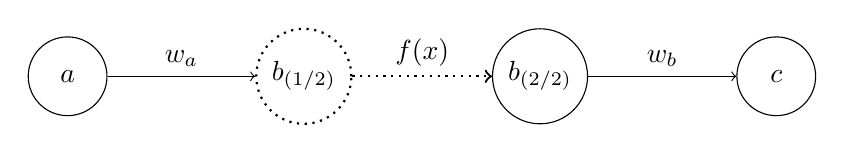
\begin{tikzpicture}[x=3cm]
        \tikzset{
            netnode/.style={circle,draw=black,minimum size=1cm},
        }
        \node[netnode] (a) at(0,0) {$a$};
        \node[netnode,dotted,thick] (b1) at(1,0) {$b_{(1/2)}$};
        \node[netnode] (b2) at(2,0) {$b_{(2/2)}$};
        \node[netnode] (c) at(3,0) {$c$};

        \draw[->] (a) -- node[above] {$w_a$} (b1);
        \draw[->,dotted,thick] (b1) -- node[above] {$f(x)$} (b2);
        \draw[->] (b2) -- node[above] {$w_b$} (c);
    \end{tikzpicture}
    \caption{Neuronenkette}
\end{figure}

Um herauszufinden, wie eine Änderung von $w_a$ sich auf den Wert des Neurons $c$
auswirkt, kann die \emph{Chainingeigenschaft} genutzt werden (TODO: cite).
Diese kann leicht gezeigt werden, denn es gilt:

\begin{align*}
    c         & = b_{(2/2)}\cdot w_b \\
    b_{(2/2)} & = f(b_{(1/2)})       \\
    b_{(1/2)} & = a\cdot w_a
\end{align*}

(TODO: berechnung)